\documentclass[11pt]{article}
\usepackage[letterpaper,margin=0.85in]{geometry}
\usepackage{graphicx,booktabs,longtable,amsmath,xurl,enumitem,caption}
\usepackage[hidelinks]{hyperref}
\setlist{itemsep=2pt}
\newcommand{\step}[1]{\subsection*{#1}}
\title{\textbf{RC Catamaran 1\,m: Build Manual}\\\large Build-first boat and the v2.2 foiling kit}
\author{Filip Maleev}
\date{September 2026}
\begin{document}
\maketitle
\begin{center}
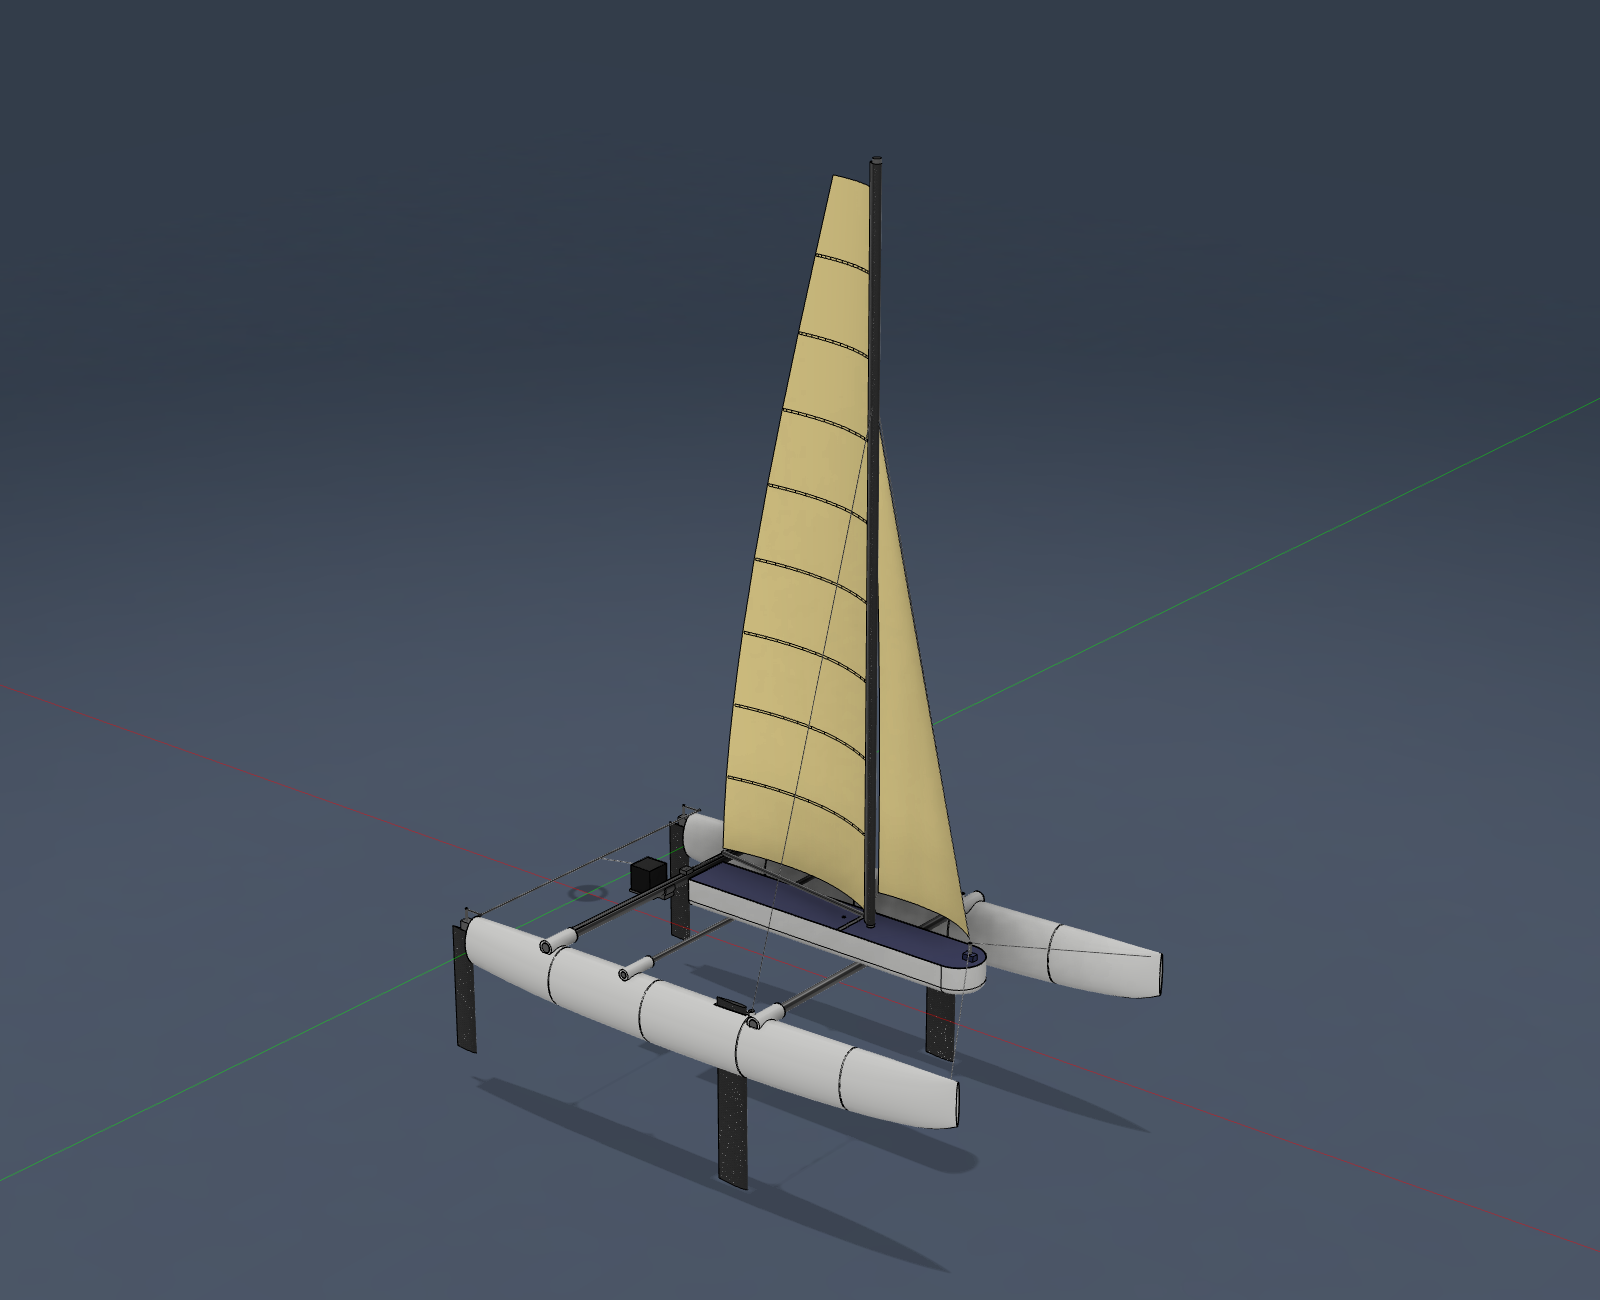
\includegraphics[width=0.48\linewidth]{../images/build_first_v1.4.png}\hfill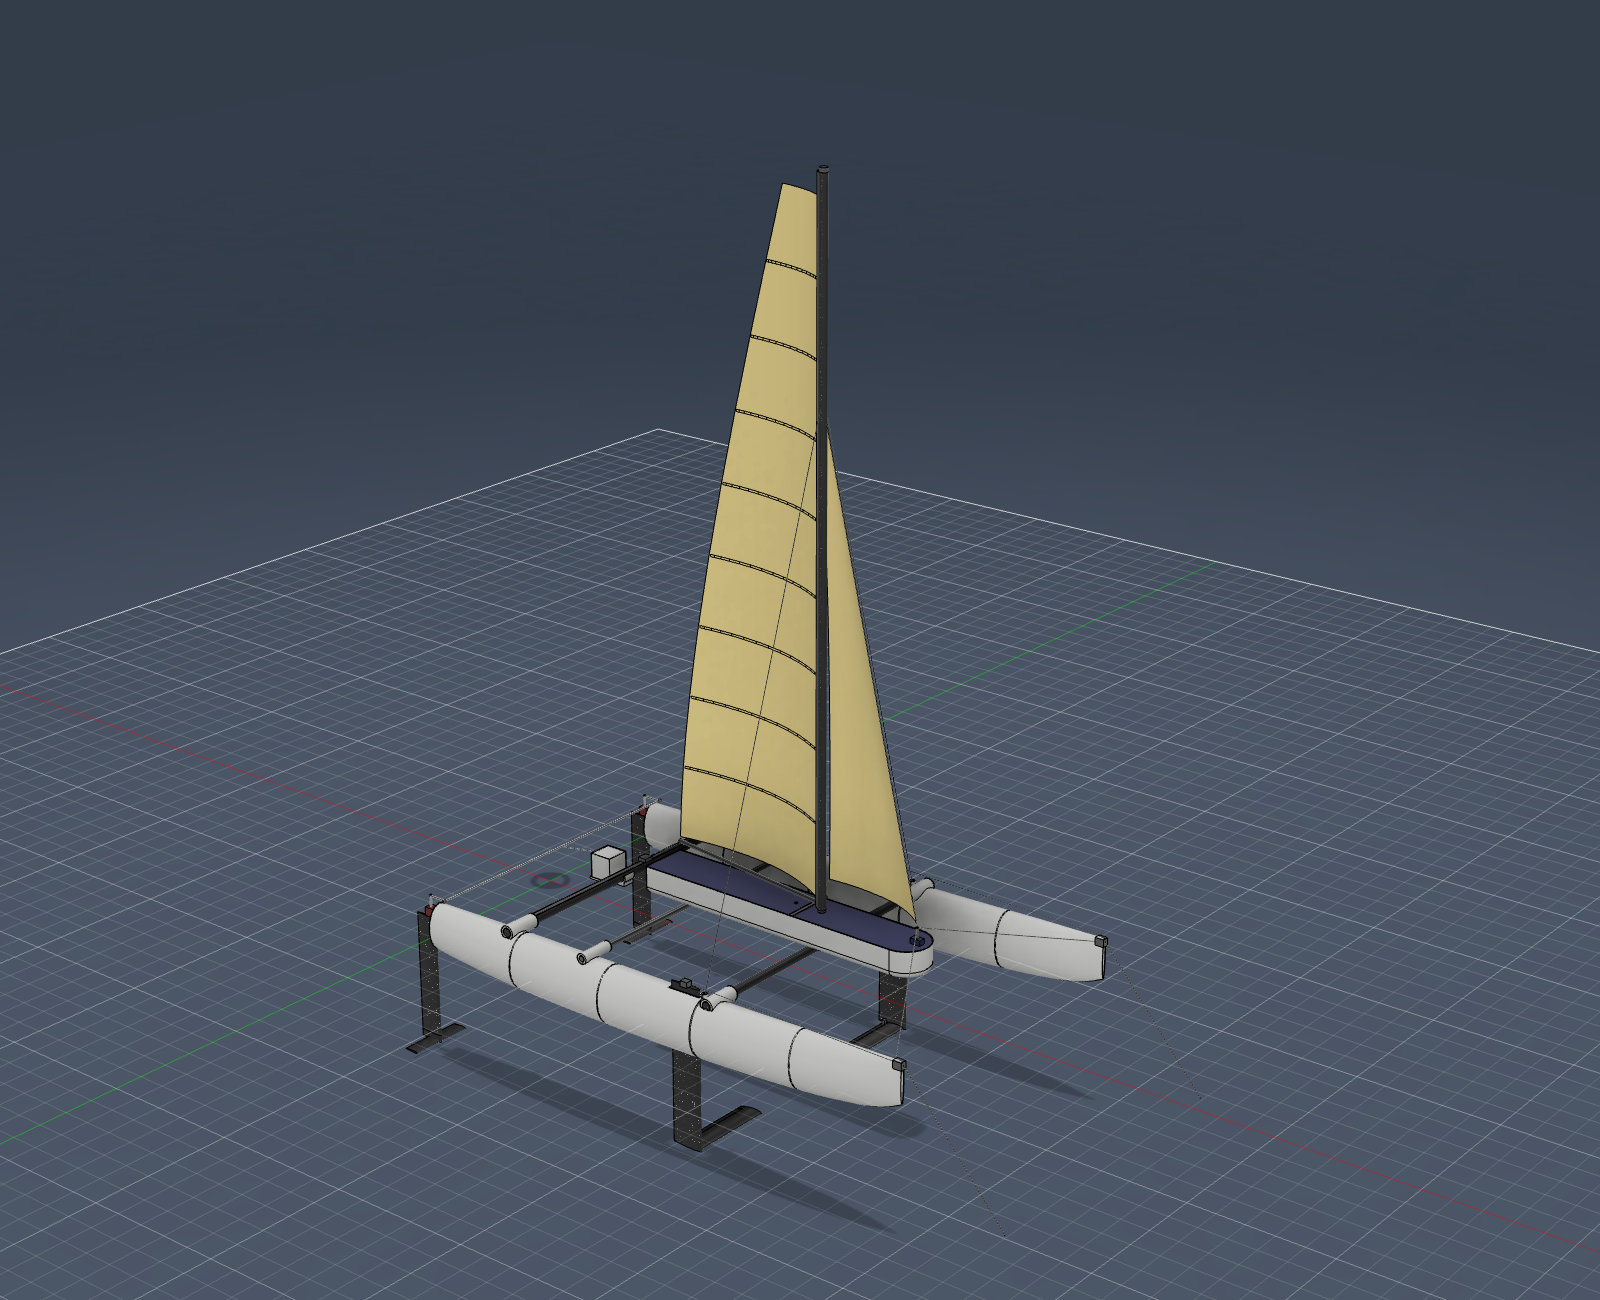
\includegraphics[width=0.48\linewidth]{../images/foiling_v2.2.png}
\end{center}

\section{What you are building}
A 1\,m catamaran with a beach-cat rig: a square-top, fully battened main on a rotating wing mast, a jib on a forestay bridle, and three sail controls (jib sheet, traveler, mainsheet tension) on three servos. Build the boat with daggerboards first (the \emph{build-first} version, 2037\,g ready to sail). Once it sails well, the foiling kit replaces the daggerboards with L-foils, adds wand-driven flaps for ride-height control, and puts T-foil elevators on the rudders (2242\,g).

Predicted, not yet measured: the build-first boat does 2.67\,m/s on a beam reach in 8\,kn of wind. The foiling version flies from about 7.2\,kn on a beam reach and 10.7\,kn at 60$^\circ$ to the wind, and does 4.65\,m/s on a beam reach in 12\,kn.

\textbf{Build the 0.6\,m Mini Cat first} (its own manual). Many steps here assume you have done them once at that size.

\section{What it costs}
Build-first boat \textbf{\$381.02}; foiling kit \textbf{\$101.17} more. Prices were read on retailer pages in September 2026 (sources at the end). Shipping, tax, a NiMH charger, the printer and hand tools (including a 0.9\,mm hex key for the elevator trim screws) are not included. The FS-i6X radio and 4xAA pack from the Mini Cat carry over.

{\small
\begin{longtable}{p{1.6cm}p{4.4cm}p{6.6cm}cr}
\toprule
Group & Item & Use & Qty & Total \\
\midrule
\multicolumn{5}{l}{\textbf{Build-first boat}}\\
Radio & FlySky FS-i6X + FS-iA6B receiver & 4 channels used: rudder, traveler, jib, mainsheet & 1 & \$69.99 \\
Radio & AA alkaline x4 & transmitter power & 1 & \$2.99 \\
Servos & JX W4505-4T sail winch servo & traveler (about 231 mm of car travel, rig model) & 1 & \$11.13 \\
Servos & JX W4505-2T sail winch servo & jib sheet (about 93 mm of sheet, rig model) & 1 & \$11.13 \\
Servos & Feetech FS5115M standard servo & mainsheet tension & 1 & \$32.06 \\
Servos & MG90S metal-gear micro servo & rudders via pushrod + tie bar & 1 & \$2.59 \\
Power & Panasonic eneloop AA 2000 mAh, 4-pack & receiver pack (4.8 V) & 1 & \$12.75 \\
Power & Traxxas 4-cell AA holder with switch (TRA1523) & receiver battery box + on/off & 1 & \$4.00 \\
Printed & PETG filament 1 kg & hulls, pod, lid, rudder-servo bracket and cover, rudders, boards, tracks, cars (~1.4 kg used, 1 m manual print list) & 2 & \$27.98 \\
Carbon & Carbon tube 16 x 14 mm x 1 m & two 600 mm crossbeams & 2 & \$32.56 \\
Carbon & Carbon tube 12 x 10 mm x 1 m & two-piece mast (1.3 m) & 2 & \$24.52 \\
Carbon & Carbon tube 10 x 8 mm x 1 m & mast joiner spigot (150 mm) and pod beam (600 mm) & 1 & \$16.15 \\
Carbon & Carbon tube 8 x 7 mm x 1 m & boom (345 mm) & 1 & \$17.20 \\
Carbon & Carbon rod 1.2 mm x 2 m & 8 battens & 1 & \$5.25 \\
Hardware & Music wire 0.156 in & rudder stocks, tie bar & 2 & \$9.98 \\
Hardware & Music wire 0.093 in & rudder pushrod, bent turning eyes for the control lines & 1 & \$3.99 \\
Hardware & Du-Bro micro pushrod system & clevises & 1 & \$8.55 \\
Sails & Icarex PC31 ripstop polyester, 1 m & main + jib (0.40 m2) & 1 & \$21.99 \\
Sails & Ripstop sail tape 2 in, half roll & luff, batten pockets, corners & 1 & \$24.00 \\
Rigging & Braided PE line 30 lb & stays, bridle, sheets & 1 & \$14.43 \\
Adhesives & BSI 5-minute epoxy 9 oz & hull joints, beams, fittings & 1 & \$22.99 \\
Adhesives & BSI gap-filling CA 1/2 oz & small parts & 1 & \$4.79 \\
\midrule
\multicolumn{5}{l}{\textbf{Foiling kit}}\\
Printed & PETG filament 1 kg & L-foil, elevator and flap cores, bellcranks (~400 g) & 1 & \$13.99 \\
Carbon & Unidirectional carbon tape 2 in x 12 ft & spar caps: 4 layers per face on struts, wings, elevators & 2 & \$39.90 \\
Adhesives & EL2 laminating epoxy 500 g & wet-out of the caps & 1 & \$20.70 \\
Carbon & Carbon rod 1.2 mm x 1 m & flap hinge pins & 1 & \$3.47 \\
Carbon & Carbon rod 2 mm x 1 m & two 300 mm ride-height wands, two elevator pivot pins & 1 & \$8.85 \\
Hardware & Music wire 0.047 in & wand-to-flap pushrods & 1 & \$3.99 \\
Hardware & Du-Bro micro pushrod system & clevises for the flap linkage & 1 & \$8.55 \\
Hardware & M2 x 6 mm stainless set screw, cup point (Bolt Depot 8697) & elevator trim screws, two per trim pod & 4 & \$1.72 \\
\bottomrule
\end{longtable}}

\section{Printing}
PETG throughout. The hull and pod segments are real 0.8\,mm skins with the bulkheads built in: slice them with 2 perimeters and 0\,\% infill, so each segment prints as a sealed compartment. Print the rudder blades, daggerboards, foil cores, flaps and trim pods solid (100\,\% infill is our recommendation for stiffness, not a tested setting). Filament below is for solid parts at 1.27\,g/cm$^3$ and for the skins as modelled.

{\small
\begin{longtable}{lcrr}
\toprule
STL file (folder \texttt{stl/}) & Qty & Size (mm) & PETG (g) \\
\midrule
\multicolumn{4}{l}{\textbf{Boat}}\\
\url{Hull_Port_Seg_1_x0_200.stl} & 1 & 200 x 117 x 82 & 69 \\
\url{Hull_Port_Seg_2_x200_400.stl} & 1 & 200 x 120 x 84 & 80 \\
\url{Hull_Port_Seg_3_x400_600.stl} & 1 & 200 x 117 x 81 & 91 \\
\url{Hull_Port_Seg_4_x600_800.stl} & 1 & 200 x 118 x 83 & 78 \\
\url{Hull_Port_Seg_5_x800_1000.stl} & 1 & 200 x 115 x 65 & 54 \\
\url{Hull_Stbd_Seg_1_x0_200.stl} & 1 & 200 x 117 x 82 & 69 \\
\url{Hull_Stbd_Seg_2_x200_400.stl} & 1 & 200 x 120 x 84 & 80 \\
\url{Hull_Stbd_Seg_3_x400_600.stl} & 1 & 200 x 117 x 81 & 91 \\
\url{Hull_Stbd_Seg_4_x600_800.stl} & 1 & 200 x 118 x 83 & 78 \\
\url{Hull_Stbd_Seg_5_x800_1000.stl} & 1 & 200 x 115 x 65 & 54 \\
\url{Pod_Lid_Seg_1_x270_380.stl} & 1 & 110 x 90 x 1 & 15 \\
\url{Pod_Lid_Seg_2_x380_600.stl} & 1 & 220 x 90 x 1 & 30 \\
\url{Pod_Lid_Seg_3_x600_840.stl} & 1 & 240 x 90 x 11 & 34 \\
\url{Pod_Shell_Seg_1_x270_380.stl} & 1 & 110 x 90 x 57 & 47 \\
\url{Pod_Shell_Seg_2_x380_600.stl} & 1 & 220 x 90 x 54 & 92 \\
\url{Pod_Shell_Seg_3_x600_840.stl} & 1 & 240 x 90 x 60 & 79 \\
\url{Rudder_Servo_Bracket.stl} & 1 & 73 x 46 x 26 & 23 \\
\url{Rudder_Servo_Cover.stl} & 1 & 45 x 44 x 43 & 14 \\
\url{Rudder_Blade_x2.stl} & 2 & 226 x 45 x 5 & 96 \\
\url{Daggerboard_x2.stl} & 2 & 325 x 60 x 7 & 244 \\
\midrule
\multicolumn{4}{l}{\textbf{Foiling kit}}\\
\url{Foil_Core_L_Port.stl} & 1 & 296 x 164 x 60 & 125 \\
\url{Foil_Core_L_Stbd.stl} & 1 & 296 x 164 x 60 & 125 \\
\url{Foil_Core_Elevator_x2.stl} & 2 & 120 x 28 x 3 & 14 \\
\url{Foil_Flap_x2.stl} & 2 & 146 x 11 x 3 & 6 \\
\url{Elevator_Trim_Pod_x2.stl} & 2 & 45 x 14 x 9 & 7 \\
\url{Foiling_Rudder_Extension_x2.stl} & 2 & 45 x 5 x 3 & 1 \\
\bottomrule
\end{longtable}}
\noindent Total: about 1421\,g for the boat and 279\,g for the foiling kit, before supports and failed prints.

\noindent\textbf{Not yet printable.} These small fittings are blocks in the CAD model that stand in for their mass and position; each needs to be designed before it can be printed: gudgeons, traveler and jib tracks and cars, mast cap, bridle post, and, for the foiling kit, the wand pivots, strut bellcranks and flap horns.

\section{Building the boat}
\step{1. Hulls}
\begin{enumerate}
\item Print the ten hull segments. Each ends in half of a bulkhead; the faces meet flat.
\item Epoxy the segments of each hull face to face in order (x = 0 is the transom), keeping the keel line straight on a flat surface.
\item Seal test: submerge each hull in a tub for 10 minutes and look for bubbles or water. Each segment is a separate compartment, so one leak floods only one.
\end{enumerate}
\step{2. Crossbeams and pod beam}
\begin{enumerate}
\item Cut two 600\,mm crossbeams from the 16\,x\,14\,mm tube, and a 600\,mm pod beam plus the 150\,mm mast joiner from the 10\,x\,8\,mm tube (wear a mask when cutting or sanding carbon).
\item Epoxy the crossbeams into the front and rear sockets of both hulls and the pod beam into the third socket, with the hulls parallel and the beams square.
\end{enumerate}
\step{3. Pod and electronics}
\begin{enumerate}
\item Bond the three pod shell segments and the three lid segments. The pod snaps onto the front beam and the pod beam.
\item Fit the two sail winches (traveler: 4-turn; jib sheet: 2-turn) and the mainsheet servo on their rails. The winches hang by their ears in 4--6\,mm wells. JX does not publish the winch's ear height; the rails use the FS5115M value (27.3\,mm above the case bottom). If a winch case touches the bottom of its well first, shim under the ears.
\item Receiver and the 4xAA pack with its switch go in the pod. The two traveler lines and the mainsheet tail leave the pod through the three holes in its transom and run aft under the rear beam to turning eyes on its front face, bent from the 0.093\,in wire.
\end{enumerate}
\step{4. Rudders}
\begin{enumerate}
\item Rudder stocks from the 0.156\,in music wire, through the printed blades (pivot at 25\,\% chord). The gudgeons that hold them are still placeholders in the CAD (Section 3).
\item Snap the rudder-servo bracket onto the rear beam from below, centred between the hulls, and epoxy it so it cannot rotate. The MG90S hangs by its ears on the bracket's rails, aft of the beam, under the printed cover. The pushrod (0.093\,in wire, Du-Bro clevises) runs from the slot in the cover to the tie bar, which joins the two tiller arms.
\end{enumerate}
\step{5. Rig}
\begin{enumerate}
\item Mast: the two 12\,x\,10\,mm tubes joined by the 150\,mm spigot, 1298\,mm overall. Hounds 928\,mm above the mast foot.
\item Standing rigging from the 30\,lb braided line (lengths between fittings): forestay 873\,mm, each bridle leg 336\,mm, each shroud 974\,mm. Add your own allowance for knots.
\item Boom: 345\,mm of the 8\,x\,7\,mm tube. Traveler track on the rear beam, jib track on the pod lid.
\end{enumerate}
\step{6. Sails}
\begin{enumerate}
\item Print the 1:1 patterns (\texttt{manual\_1m/sail\_patterns\_1m\_1to1.pdf}, a single tall sheet: a copy shop's plotter, or tile it) and check the 100\,mm scale bar.
\item Cut the main (foot 345, luff 1190, head 105\,mm) and the jib (foot 221, luff 849\,mm) from the Icarex. Tape the edges, corners and eight batten pockets with the sail tape.
\item Battens from the 1.2\,mm carbon rod, bottom to top (mm): 331, 318, 300, 276, 249, 216, 180, 140. How the luff attaches to the wing mast is not detailed in the CAD: a sleeve, as on the Mini Cat, is one option.
\end{enumerate}
\step{7. Mainsheet routing}
The traveler car moves up to 236\,mm across the beam, far more line than the mainsheet servo can take up, so the car must not pull on the mainsheet. Dead-end the mainsheet at the port end of the rear beam, run it through the traveler car, up to the boom and back down, then out of the other side of the car to a turning block at the starboard end and back under the beam into the pod. Moving the car then shortens one side of the sheet exactly as much as it lengthens the other.
\step{8. Radio setup}
\begin{enumerate}
\item Bind the receiver and assign four channels: rudder, traveler, jib sheet, mainsheet tension.
\item Traveler winch: set its end points so the car runs the full track (about 231\,mm of car travel in the rig model) without hitting the ends. Jib winch: about 93\,mm of sheet from sheeted in to eased. Mainsheet servo: set its end points by eye, flattest leech without stalling the servo.
\item Rudder: stick right, bow right. The linkage gives $\pm18^\circ$ of rudder.
\item Failsafe: rudders centred and sheets eased on signal loss.
\end{enumerate}
\step{9. Balance and float test}
Rigged, the build-first boat should balance 457\,mm forward of the transoms (move the battery to correct it). Float it and check both hulls sit level; leave it 10 minutes and check the pod and hulls for water.

\section{The foiling kit}
Fit the kit only after the build-first boat sails well.
\step{10. Foil cores and carbon caps}
\begin{enumerate}
\item Print the L-foil cores (port and starboard are mirror images), the elevator cores and the flaps. The cores have 0.5\,mm deep, 25\,mm wide recesses on both faces of the strut, the wing and the elevator for the carbon caps.
\item Split the 2\,in unidirectional tape lengthwise into 25\,mm strips and lay 4 layers into each recess with the laminating epoxy, fibres along the span; the caps finish flush with the section. The caps use about 4.5\,m of the 7.3\,m of tape.
\item The strut has a 2.4\,mm channel for the flap pushrod (0.047\,in wire); keep it clear of epoxy.
\end{enumerate}
\step{11. Flaps}
The flap is the aft 25\,\% of each wing (11\,mm), from 10\,mm inside the tip to the strut. It hinges on 1.2\,mm carbon pins on its leading edge, 34\,mm behind the wing's leading edge. The CAD does not model the hinge holes: drill them on that line at each end of the flap. The flap must swing $\pm15^\circ$ freely.
\step{12. Ride-height linkage}
One wand per hull, 300\,mm of 2\,mm carbon rod, hinged at the bow. It drives its flap through a deck pushrod, a bellcrank and the pushrod inside the strut. The linkage must give:
\begin{itemize}
\item \textbf{zero flap} with the wand 49$^\circ$ below the deck line (the design ride height, hinge about 226\,mm above the water);
\item \textbf{1.5$^\circ$ of flap per degree of wand}, wand down giving flap down;
\item the full $\pm15^\circ$ of flap without binding.
\end{itemize}
The wand pivots, bellcranks and flap horns are placeholders in the CAD (Section 3): design them to these three numbers.
\step{13. Elevators and trim pods}
\begin{center}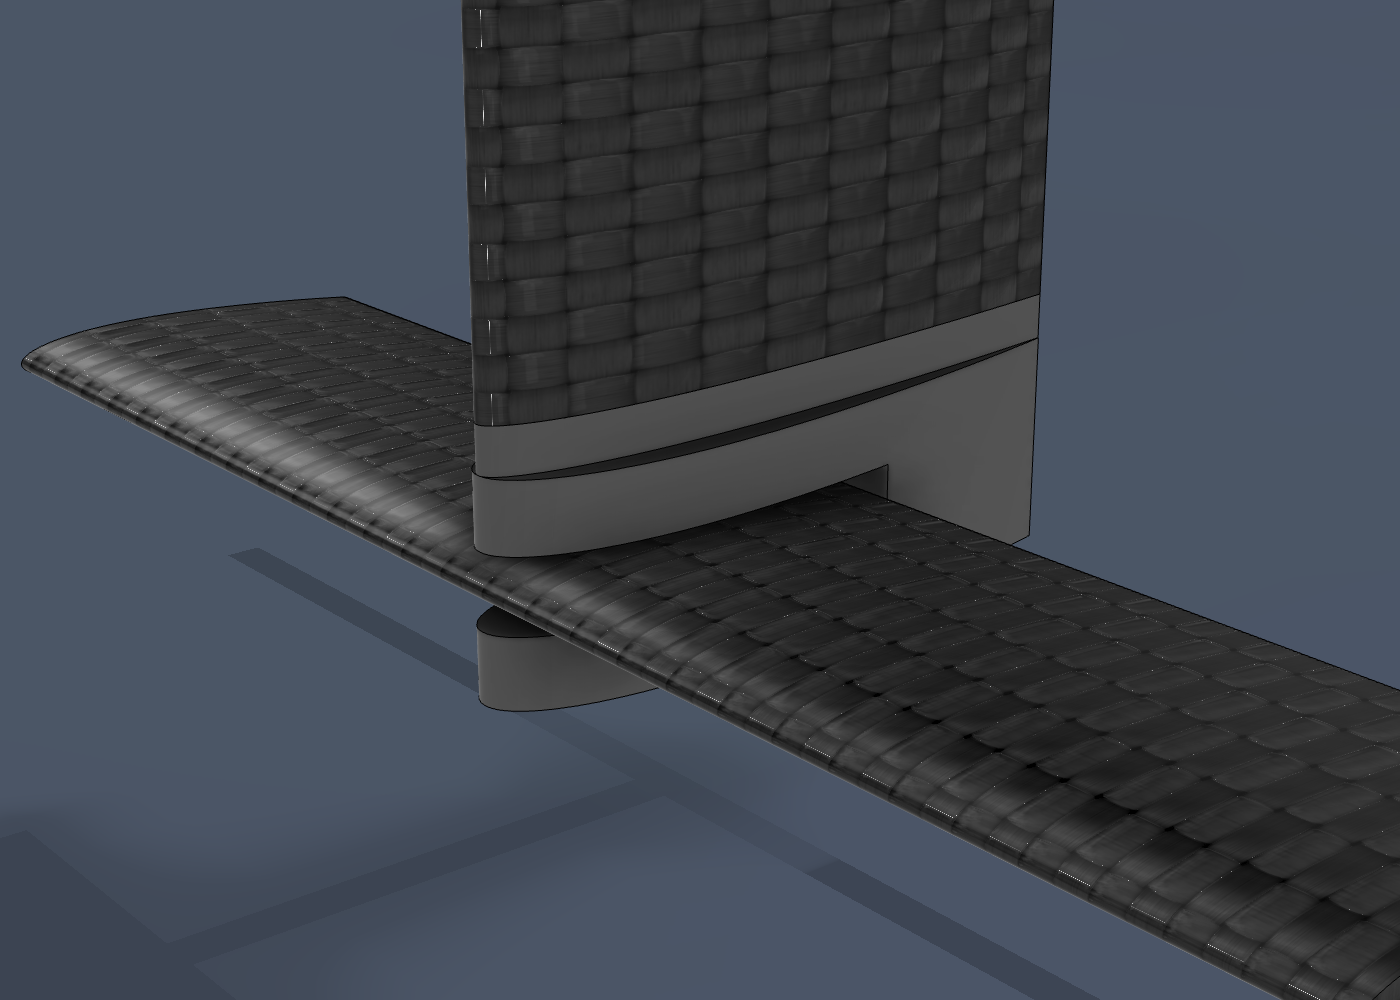
\includegraphics[width=0.6\linewidth]{../images/elevator_trim_pod.png}\end{center}
\begin{enumerate}
\item Bond a 3\,mm extension and then a trim pod under each rudder blade; the pod's slot is at the elevator's height.
\item Slide the elevator through the slot and pin it at its quarter chord with a 10\,mm piece of the 2\,mm carbon rod.
\item Two M2 set screws, one from above and one from below, clamp it 12\,mm behind the pin. One turn moves the elevator about $1.9^\circ$. Set $-1^\circ$ (nose down) to start.
\end{enumerate}
\step{14. Fit and set up}
\begin{enumerate}
\item Replace the daggerboards with the L-foils in the same trunks. Main wing incidence $+1.5^\circ$.
\item Rebalance: the foiling boat should balance 462\,mm forward of the transoms, 2242\,g in total.
\item Run the bench checks and the tow test in \texttt{testing/RC\_Foiling\_Cat\_Tow\_Test\_Plan.pdf} before sailing on the foils.
\item First flights: take off on a beam reach, where the foils have enough roll authority, then head up. Near take-off the leeward hull may keep touching; that is expected.
\end{enumerate}

\section*{Price sources (read September 2026)}
{\small\begin{itemize}
\item HobbyTown: \url{https://www.hobbytown.com/flysky-i6x-6channel-afhds-2a-air-radio-system-w-ia6b-receiver-fsy-i6xia6b/p1674181}
\item HobbyTown (EcoPower AA x4 add-on): \url{https://www.hobbytown.com/flysky-fsgt2e-2channel-transmitter-w-fsa3-receiver-fsy-fs-gt2ea3/p1592822}
\item AliExpress: listed \$5.79 at 48\% off; full price used: \url{https://www.aliexpress.com/item/1005003265131874.html}
\item Pololu: \url{https://www.pololu.com/product/3426}
\item Waveshare: \url{https://www.waveshare.com/mg90s-servo.htm}
\item MicroBattery: \url{https://www.microbattery.com/panasonic-bk-3mcca4ba-eneloop-aa-2100-cycle-ni-mh-pre-charged-rechargeable-batteries-4-pack80.html}
\item HobbyTown: \url{https://www.hobbytown.com/traxxas-4cell-aa-battery-holder-w-switch-cover-tra1523/p49945}
\item Elegoo US: \url{https://us.elegoo.com/products/rapid-petg-filament-1-75mm-colored-1kg}
\item Wind Catcher RC (price from search listing, page not reachable from here): \url{https://windcatcherrc.com/product/carbon-fiber-tube-16mm-x-14mm-x-1000mm/}
\item RMRC: \url{https://www.readymaderc.com/products/details/carbon-fiber-tube-12mm-x-10mm-1m-long}
\item CST CS-525 1M: \url{https://www.cstsales.com/Carbon_Fiber_Tubes.html}
\item CST CS-316 2M: \url{https://www.cstsales.com/carbon_rods.html}
\item K\&S 0.156 in x 12 in: \url{https://ksmetals.com/collections/12-long-music-wire}
\item HobbyTown: \url{https://www.hobbytown.com/dubro-pushrod-system-micro-dub847/p29360}
\item Jones Airfoils, per metre (138 cm wide): \url{https://jonesairfoils.com/products/icarex}
\item kiteboarding.com: \$15.00 base + \$9.00 half roll: \url{https://kiteboarding.com/proddetail.asp?prod=ripstop_2inch}
\item Walmart, PowerPro 30 lb x 150 yd (read 2026-09-24; the original eBay listing had ended): \url{https://www.walmart.com/ip/PowerPro-Braided-Fishing-Line-30lb-x-150yd-ylw-21100300150Y/17117880}
\item HobbyTown: \url{https://www.hobbytown.com/bob-smith-industries-quickcure-5-minute-epoxy-9o-bsi202/p37082}
\item HobbyTown: \url{https://www.hobbytown.com/bob-smith-industries-instacure-gap-filling-ca-1-2oz-bsi106/p37055}
\item CST CU-379: 2 in unidirectional carbon, 0.005 in, 12 ft: \url{https://www.cstsales.com/heat_tack.html}
\item Easy Composites EL2, 500 g kit: \url{https://www.easycomposites.us/el2-epoxy-laminating-resin}
\item Bolt Depot, per piece (read 2026-09-25): \url{https://boltdepot.com/Product-Details?product=8697}
\end{itemize}}
\end{document}
